\chapter{Noise Generation}
\label{NoiseGen}
noise generation is one of the most essential topic in procedural content generation. Noise is often used in computer graphics and special effects, but is also used to randomly create or modify procedurally generated worlds. Noise generation can be a very complicated topic to fully understand. We will in this chapter look into some of the most commonly known noises as well as how to use them and manipulate them.


\section{Perlin Noise}

Perlin noise is one of the most common used noises in computer graphics and special effect. Perlin noise was originally created by Ken Perlin\cite{KenPerlin} in 1985 while working on the movie Tron\cite{perlinnoise}. Perlin noise is also the noise that often is used or adapted upon to create other sorts of noises, or manipulating with noises.

As we have mentioned earlier we will use libnoise for this project and will there by not implement our own perlin noise, however this section should provide the idea about how to implement your own perlin noise, as well as how perlin noise in general works.

Perlin noise is created by adding multiple layers of noise together with different amplitude, the amount between the highest and the lowest peak value, and frequency, how often the value is changed\cite{perlinnoise2}. Values are randomly generated within the amplitude and frequency range as the example in \figref{fig:1DNoise} show. The final result from adding all the layers together will give a smooth noise pattern which then can be used to define low and high values. To demonstrate the process we have 6 layers of noise in \figref{fig:1DNoise}, and when taking the sum of all graphs we end up with a graph shown in \figref{fig:1DNoiseResult}

\begin{figure}[H]
	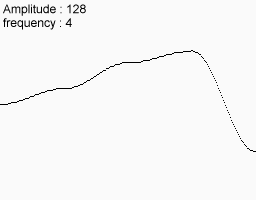
\includegraphics[width=0.32\linewidth]{img/noise_a}
	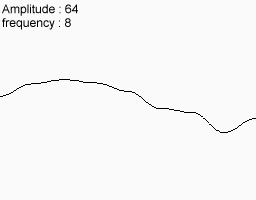
\includegraphics[width=0.32\linewidth]{img/noise_b}
	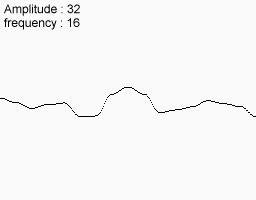
\includegraphics[width=0.32\linewidth]{img/noise_c}
	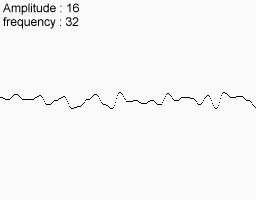
\includegraphics[width=0.32\linewidth]{img/noise_d}
	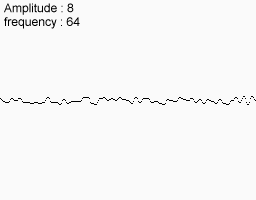
\includegraphics[width=0.32\linewidth]{img/noise_e}
	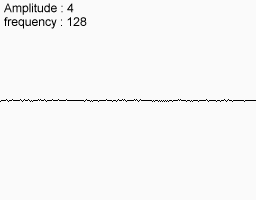
\includegraphics[width=0.32\linewidth]{img/noise_f}
	\centering
	\caption{6 graphs showing different layers of noise with the amplitude getting halved and frequency doubled for every new layer to finally create the result seen in \figref{fig:1DNoiseResult} Images used is taken from \cite{perlinnoise2}.}
	\label{fig:1DNoise}
\end{figure}
\begin{figure}[H]
	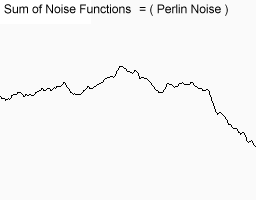
\includegraphics[width=0.5\linewidth]{img/perlin1}
	\centering
	\caption{The final graph result from the sum of all of the graphs shown in \figref{fig:1DNoise}. The image used is taken from \cite{perlinnoise2}.}
	\label{fig:1DNoiseResult}
\end{figure}

The exact same idea can be adapted to create 2 dimensional noise. In \figref{fig:2DNoise} we see the exact same that happened in \figref{fig:1DNoise} but in a 2 dimensional space rather than in 1 dimension. We have 6 different noise maps with different amplitude and frequency which is combined into a single noisemap which should give a smooth gradient transition between high and low values. All the black areas is typically representing the lowest values and white represent the highest values however, in \figref{fig:2DNoise} case purple represents the high values.

\begin{figure}[H]
	
\includegraphics[width=0.135\linewidth]{img/perlin_a}
	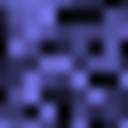
\includegraphics[width=0.135\linewidth]{img/perlin_b}
	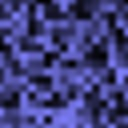
\includegraphics[width=0.135\linewidth]{img/perlin_c}
	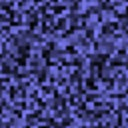
\includegraphics[width=0.135\linewidth]{img/perlin_d}
	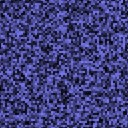
\includegraphics[width=0.135\linewidth]{img/perlin_e}
	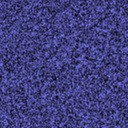
\includegraphics[width=0.135\linewidth]{img/perlin_f}
	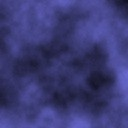
\includegraphics[width=0.135\linewidth]{img/p_128}
	\centering
	\caption{The images show layers of 2 dimensional noise with the frequency getting larger with the leftmost image being the lowest frequency. The Rightmost image is the final noise generated from the 6 other images. Images used is taken from \cite{perlinnoise2}.}
	\label{fig:2DNoise}
\end{figure}

Perlin noise offers multiple parameters that we can change, to modify the output noise. The first and most important is octaves which defines how many layers of noise should be created to produce the final result. In \figref{fig:1DNoise} and \figref{fig:2DNoise} the octaves is 6, as there is 6 noise maps that is used to generate the final result. We also need a parameter to define our starting frequency, and the frequency multiplier, which is often referred to as persistence. In \figref{fig:1DNoise} we have a persistence of 2 as the frequency is double on each octave and the amplitude halved. In libnoise persistence does however only control the amplitude, and libnoise introduce yet another parameter called lacunarity which in libnoise is used as the frequency multiplier\cite{libnoisePerlin}.

The last thing needed to make perlin noise is an interpolation function. Interpolation is a way of connecting the randomly generated points to each other. The first is linear interpolation, which is demostrated in \figref{fig:1a}, the connections is direct and the result may not be very realistic. Too improve the result even more we could use a cosine interpolation as seen in \figref{fig:1b}. We now have a somewhat realistic curves, but we can improve the curve even more by making a cubic interpolation as shown in \figref{fig:1c}. Cubic interpolation is often used as it provide the most realistic curves between multiple points. The last step is an optional step that can make the output noise slightly more realistic by smoothing the curve so that the peak values get reduced as can be seen in \figref{fig:1d}.


\begin{figure}[H]
	\begin{minipage}[b]{.5\linewidth}
		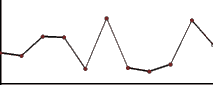
\includegraphics[width=0.95\linewidth]{img/m_inter1}
		\subcaption{Linear interpolation}
		\label{fig:1a}
		%\begin{equation*}
		%	a*(1-x) + b*x
		%	\label{linear}
		%\end{equation*} 
	\end{minipage}
	\begin{minipage}[b]{.5\linewidth}
		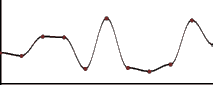
\includegraphics[width=0.95\linewidth]{img/m_inter2}
		\subcaption{Cosine interpolation}
		\label{fig:1b}
		%\begin{equation*}
		%	(1 - cos(x * \pi)) * .5
		%	\label{Cosine}
		%\end{equation*} 
	\end{minipage}
	\begin{minipage}[b]{.5\linewidth}
		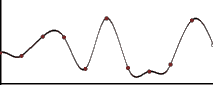
\includegraphics[width=0.95\linewidth]{img/m_inter4}
		\subcaption{Cubic interpolation}
		\label{fig:1c}
	\end{minipage}%
	\begin{minipage}[b]{.5\linewidth}
		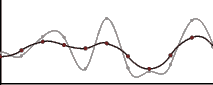
\includegraphics[width=0.95\linewidth]{img/m_inter6}
		\subcaption{Smoothed noise}
		\label{fig:1d}
		%\begin{equation*}
		%	a*(1-x) + b*x
		%	\label{linear}
		%\end{equation*} 
	\end{minipage}%

	\centering
	\caption{The images shows 3 types of interpolation. \figref{fig:1a} shows Linear interpolation, \figref{fig:1b} shows Cosine interpolation, \figref{fig:1c} shows Cubic interpolation. \figref{fig:1d} is a last optional step that smoothen the final result such that the peaks get reduced. All images used is taken from \cite{perlinnoise2}.}
	\label{fig:interpolation}
\end{figure}

Example usage of perlin noise, other than for what we already have mentioned, could be realtime generate of ocean waves, weather effect including clouds, rain, or storms.


\section{Voronoi Diagram}

\section{Fractal Noise}

\section{Rigged Noise}

\section{Manipulating noise}